\pagebreak
\fancyhf{}
\lhead{Michael Kainz}
\rhead{Seite \thepage}
\section{Software - ESP8266}
Der ESP8266 ist ein 32bit Mikrocontroller der Firma Espressif. Er besitzt ein integriertes
WIFI-Modul und in der verwendeten Version 1MB Flashspeicher.
\begin{figure}
    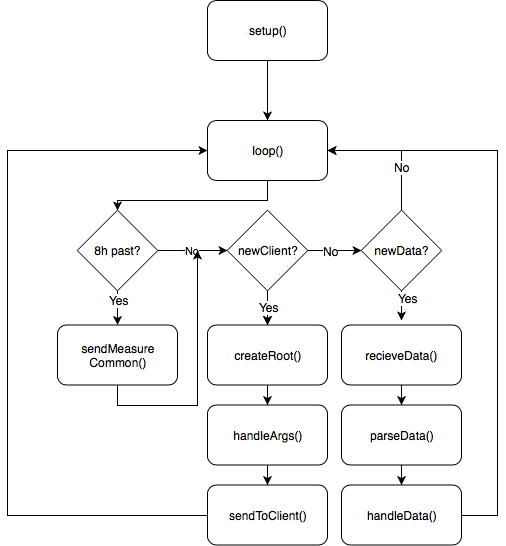
\includegraphics[width=\textwidth]{images/flow}
    \caption{Ablauf des ESP8266 Programms}
\end{figure}

\begin{tabular}{|l|l|}
    \hline
    Größen & Werte \\\hline
    Spannung & 2,5V..3,6V\\\hline
    Stromaufnahme & 2,5 $\mu$A..400mA\\\hline
    IO & 11..13 digitale Pins\\\hline
    Schnittstellen & SPI, UART, I$^2$C\\\hline
    Protokolle & TCP/IP v4 und v6, UDP, TCP\\\hline
    Datenrate & 150-300 kByte/s, Latenz ~10ms\\\hline

\end{tabular}

\subsection{Programmieren per Arduino IDE}
Der ESP8266 wird standardweise mit einem AT-Befehlssatz ausgeliefert, der für Modems und
Bluetooth-Module entwickelt wurde. Da der ESP8266 jedoch auch andere Aufgaben hat, als nur
dem Arduino als WIFI-Modul zu dienen, wurde eine neue Firmware geflasht und die Arduino IDE zum programmieren benutzt.
Das ermöglicht ein beschreiben des ESP8266 in C++, was es einfacher machte komplexe Abläufe
zu realisieren.
Dazu musste lediglich ein Zusatzpaket in der Arduino IDE heruntergeladen werden.

\subsection{Konfiguration}
Um den ESP8266 in Betrieb zu nehmen benötigt er die SSID und das Passwort des heimischen
Netzwerkes. Neben dem gewählten Client-Modus, kann der ESP8266 auch selbst als Server dienen.
Diese Funktion wurde nicht gewählt, da er zur Anzeige der Graphen und der Zeit eine
Internetverbindung braucht.
